\documentclass[tikz,border=2pt]{standalone}
\usepackage{tikz}
\usepackage{lmodern}
\usetikzlibrary{calc,decorations.pathreplacing}

% Visual conventions follow the existing MRNC TikZ pictures: ordinary
% components use TikZ's normal 0.4pt stroke, with compact TeX labels.
\tikzset{
  nu fibre/.style={
    x=0.78cm,
    y=0.78cm,
    line width=0.4pt,
    line cap=round,
    line join=round
  },
  nu label/.style={
    font=\scriptsize,
    inner sep=1pt
  },
  nu annotation/.style={
    font=\scriptsize,
    inner sep=1pt
  },
  nu dots/.style={
    font=\small,
    inner sep=0pt
  }
}

\begin{document}
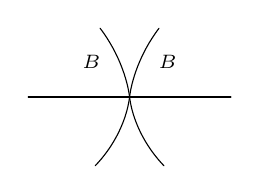
\begin{tikzpicture}[nu fibre]
  \draw (-1.65,0) -- (1.65,0);
  \draw (-0.48,1.12) .. controls (-0.16,0.70) and (-0.03,0.25) .. (0,0)
                        .. controls (-0.03,-0.25) and (-0.16,-0.70) .. (-0.56,-1.12);
  \draw (0.48,1.12) .. controls (0.16,0.70) and (0.03,0.25) .. (0,0)
                       .. controls (0.03,-0.25) and (0.16,-0.70) .. (0.56,-1.12);
  \node[nu label] at (-0.62,0.58) {$B$};
  \node[nu label] at (0.62,0.58) {$B$};
\end{tikzpicture}
\end{document}
